\documentclass[12pt]{article}
\usepackage[utf8]{inputenc}
%\usepackage{wrapfig}
\usepackage{graphicx}
\usepackage{subcaption}
\usepackage{bm}
\usepackage{verbatim}
\usepackage{float}
\usepackage{amsmath,amsfonts}
\usepackage{braket}
\usepackage[biblabel, nomove]{cite}

\textheight=22 true cm
\textwidth= 17. true cm
\oddsidemargin=-0.5truecm
\topmargin=0.truecm


\begin{document}

\title{{\normalsize Master M1 Sciences de la Mati\`ere -- ENS de Lyon --  2021-2022} \\
{\normalsize \emph{M1 Internship Report}} \\ 
\bigskip
\bigskip
\bigskip
{\bf Characterisation of rivers at a global scale}}
\author{Khalid Aleem \\
\small 
supervised by: Dr. Nelly Pustelnik, Dr. Barbara Belletti, Prof. Patrice Abry.}

\maketitle

\abstract{We cover an automated methodology for the characterisation of rivers
  at a global scale, making use of the Landsat\cite{landsat} and
  Sentinel-2\cite{sentinel} satellite data and Google Earth
  Engine\cite{google-earth-engine} to create an automated system for the
  extraction of river indices, relying on a Python library known as
  \emph{geemap}\cite{geemap} to streamline this process. Furthermore, we apply state of the art image processing techniques to our output indices in order to
  interpolate and predict datapoints that are missing from our satellite data.
  We observe continuous changes in both the spatial and temporal morphology of
  rivers through the use of our technique. This gives us a better understanding
  of river behaviour and therefore allows us to make more accurate predictions
  about their future behaviour and study how they are impacted by both
  environmental factors (seasons, climate change) and anthropormorphic factors (cities, dams, urban developments).
While the principal focus of this paper is the river Lhasa, in the Tibet region of China, this process can be easily extended to any river through the use of the Python Toolbox available.}

\newpage
\tableofcontents

\newpage

\section{Introduction}
% PURPOSE, IMAGE ANALYSIS, INTERP -- GIVE A FULL OUTLINE OF REPORT

Fluvial morphologists typically need to manually look through satellite images in order to seek and analyse features of interest in the process of performing fieldwork.  This has limitations in two different senses. Each tile of satellite data can be on the order of hundreds of megabytes. This can therefore require on the order hundreds of gigabytes of storage space to store our satellite data for processing. Aside from the storage cost, manually looking through this data in order to identify features of interest to perform fieldwork is a very time inefficient process. As a consequence, in the past, there was too much data to analyse, fluvial morphologists would only produce a few datapoints each year.

This report covers an automated methodology for the characterisation of rivers
at a global scale, allowing us to observe the behaviour of rivers continuously through space and time. With an improved ability to characterise the river morphology, we better understand and explain both the temporal and spatial behaviour of the river. This will therefore allow us to make more accurate predictions about the behaviour of rivers in the future. 

From regularly spaced river segments (polygons) and the satellite data obtained and processed from the Google Earth Engine\cite{google-earth-engine}, we provide an automated system for the extraction of river indices. 
With recent advancements in image processing relying on variational approaches and non-smooth optimisation, we succeed to develop a new interpolation method, allowing us to recover missing data and remove noise in our extracted river indices.
% With incomplete data obtained from satellite photos, this report further provides a methodology for performing time-wise and spatial interpolation of our data, where we recover river information that was otherwise obscured by clouds or the low-frequency at which satellite images are taken.
It is now significantly easier to identify features of interest on a river, improving the ability to do fieldwork. The interpolation method has been verified with expert results and a Python Toolbox is available allowing the results to be fully reproduced.
% The interpolation method has been compared to expert results

\section{Analysis of River}
From the satellite data, we calculate river indices across the river and over time as the river varies. Variation in river morphology can occur due to environmental factors (climate change/seasonal) or anthropomorphic factors (urban developments, cities, dams) as these can alter the upstream discharge rate of the river and therefore modify its morphology downstream. 

For the case of the Lhasa river, we segment the river spatially into
2km intervals. Each 2km segment of the river is known as a \emph{dis-aggregated geographical object} (DGO). The process\cite{gee-boothroyd} of segmenting our desired river into its separate DGOs is done through the use of a geographic information system, specialised software used to view and process satellite data of rivers, such as: QGIS\cite{qgis}. 

In this report, we constrain ourselves to the Lhasa river, in the Tibetan plateau, as the morphology of the river is impacted by the environment, and therefore sensitive to climate change, and also anthropomorphically, through urban developments such as the city of Lhasa and dams. Additionally, we have the shape file (Figure \ref{fig:lhasa_shp}) pre-calculated. The shape file contains a mask of the river of the maximum water extent over the past 40 years.\cite{pekel} \\

% NOTE: Fourier Analysis?

% PLOT LANDSAT IMAGES ON DGO --> LABEL DGO NUMBERS(?)
% PUT IT NEXT TO SPATIAL VARIATION PLOT OF INDEX

\begin{figure}[H]
    \centering
    \includegraphics[width=0.7\linewidth]{res/lhasa_shp.png}
    \caption{The shape/polygon file for the Lhasa River, in Tibet, China. We can view a section of the river and, crucially, the segmentation of DGOs across its length. DGO 1 is upstream and is on the top-right of the image, DGO 77 is downstream and is on the bottom-left.}
    \label{fig:lhasa_shp}
\end{figure}

Of particular interest for the Lhasa river are the indices of river area, and braiding intensity\cite{braiding-intensity}. The braiding intensity is useful as the morphology of this river is characterised by a multi-thread channel pattern. As can be seen in (Figure \ref{fig:water_mask}). Large and sudden variations in the river area and braiding intensity are indicative of a change of discontinuity in a spatially across the river or in time. For instance, a large and rapid increase/decrease in our river area index may indicate the existence of a dam along the length of the river. These indices can be calculated directly from the satellite data, either by hand or through computer processing. In practice, our indices are extracted computationally due to the huge reduction in processing time. \\

The current state of the art methodology for extracting our river indices from each DGO involves making use of the Google Earth Engine\cite{google-earth-engine}. The Google Earth Engine (Figure \ref{fig:earth_engine}) allows us to write code in JavaScript to process satellite data on the cloud. This avoids the overhead of downloading, potentially hundreds of gigabytes, of data onto our local machine. It can then be processed using Google's computing resources which are superior for this purpose than a local machine. The use of Google Earth Engine significantly reduces the computational time for river analysis. \\

The need for a similar, but alternative system arises when we consider the fact that this procedure is not a streamlined process requiring a degree of manual intervention. Thus, it is not possible to fully automate this procedure. We must run our code, manually click \emph{run} on 77 different tasks, each representing the calculated indices for each river DGO over time for a single satellite data source (in this case Landsat). Each task produces a .csv file which is saved on Google Drive. Finally, we must download all of our data in a .zip file, and run a script on our local machine to collate the data together.

\begin{figure}[H]
    \centering
    \includegraphics[width=0.7\linewidth]{res/earthengine_js.png}
    \caption{On the left pane is the file explorer. On the middle pane is the JavaScript source code viewer. On the right pane, we see 77 different tasks needing to be run manually in order to extract our river indices data into Google Drive.}
    \label{fig:earth_engine}
\end{figure}

Instead, this entire procedure is automated through the use of the Python library \emph{geemap}\cite{geemap}. This python library makes heavy use of the Google Earth Engine API, allowing us to perform the same operations as the web version of Google Earth Engine, but we may write our code and obtain our output data directly using Python. From the river polygon file alone, we may calculate our river indices in both space and time. We may then combine our data from different satellites and post-process and interpolate our data.

\begin{figure}[H]
    \centering
    \begin{subfigure}[t]{0.45\textwidth}
        \centering
        \fbox{\includegraphics[width=2.4in]{res/dgo_5_landsat_MNDWI.png}}
        \caption{Landsat (1988)}
    \end{subfigure}
    \begin{subfigure}[t]{0.45\textwidth}
        \centering
        \fbox{\includegraphics[width=2.4in]{res/dgo_5_sentinel_MNDWI.png}}
        \caption{Sentinel-2 (2019)}
    \end{subfigure}
    \caption{The water mask (red) calculated for DGO 5 for the first image in each dataset.}
    \label{fig:water_mask}
\end{figure}

\section{Landsat and Sentinel-2 Data}
\subsection{Data sources}
The two principal sources of data come from the Landsat\cite{landsat} and Sentinel-2\cite{sentinel} satellite image collections which may be used within Google Earth Engine. The Landsat data covers a date range from 1988 to 2022 (the present), while the more recent, and higher resolution Sentinel-2 data, corrected for atmospheric conditions, starts from 2019. Both data sources are multi-spectral, containing the standard red, green and blue bands, but also crucially a short wave infrared band (SWIR). 

We observe an increase in density of datapoints at the spatial centre of our river at approximately DGO 40 (Figure \ref{fig:sparsity_landsat}). This can be attributed to the overlap of satellite tiles where the DGO cell is, as such we have multiple overlapping datapoints in this region.

% TODO: Include plots of multiplicity to show datapoint frequency...

\subsection{Cloud Threshold and Data Sparsity}
We observe that our data obtained from our Landsat and Sentinel-2 satellites are both very sparse in the time axis. For Landsat we average one datapoint for every 16 day interval, while for our Sentinel-2 data we have a datapoint for each 8 day interval (week). This correspond to the re-visit time for the sattelites used in each dataset. Our satellite data is pre-processed to obtain the cloud coverage, and images that are excessively cloudy (with a tile cloud coverage exceeding 80\%) are discarded. The large gaps shown in our merged plot (Figure \ref{fig:sparsity_merged}) are a key feature of the data sparsity. The regularity of missing data in the months of July-August each year is indicative of monsoon season, where there is likely too much cloud coverage on our satellite tile to extract any information about the river. 
\begin{figure}[H]
    \centering
    \includegraphics[width=0.9\textwidth]{res/sparsity_landsat.png}
    \caption{There exists a {+} for each datapoint in space (DGO number) and time where the river indices exist. Landsat (Blue), Sentinel-2 (Orange). We observe that it is only after 2019 where river indices can be extracted from both datasets.}
    \label{fig:sparsity_landsat}
\end{figure}

\begin{figure}[H]
    \centering
    \includegraphics[width=0.9\textwidth]{res/sparsity_merged.png}
    \caption{A zoomed image of (Figure \ref{fig:sparsity_landsat}). We restrict our time axis to that of the Sentinel-2 (orange) data, allowing us to see how our second satellite allows us to fill in the gaps of our more sparse Landsat (blue) data.}
    \label{fig:sparsity_merged}
\end{figure}

% TODO: Quantities of interest
\subsection{Calculation of the Water Mask}
% Calculation of water mask. LANDSAT/SENTINEL channels
For the case of both Landsat and Sentinel-2 our modified normalised water index (MNDWI)\cite{mndwi} is calculated from our Green band, and short wave infrared (SWIR) band as follows:
$$\text{MNDWI} = \frac{\text{Green} - \text{SWIR}}{\text{Green} + \text{SWIR}}$$
We say that a pixel consists of water in the situation that $\text{MNDWI} > 0$, a process known as MNDWI thresholding\cite{mndwi}. This allows us to calculate a water mask (Figure \ref{fig:water_mask}), where each pixel is labelled as 0 or 1 depending on whether the cell is water or not. This is crucial for determining which pixels compose the river, and which do not, within each of our DGO cells.


\subsection{Calculation of the River Indices}
Finally, we cover the calculation of our river indices from our water mask. For the Lhasa river, the braiding intensity is an important quality used in characterising its morphology. For each DGO and each time, we have a water mask. The Google Earth Engine provides us with the capacity to rapidly compute the geometry, smoothed area and perimeter, of our water mask. After eliminating regions of our water mask that are too small (noise), we calculate the smoothed perimeter and smoothed area of our water mask. Our smoothed area provides us with our area index directly. Our braiding intensity (Figure \ref{fig:braiding}) may be calculated from our total smoothed perimeter of our water mask and reach length, the width of our DGO (2km for the Lhasa river segments).
$$ \text{BRAIDING\_INTENSITY} = \frac{TOTAL\_PERIMETER/2}{REACH\_LENGTH} $$

\begin{figure}[H]
    \centering
    \includegraphics[width=0.7\linewidth]{res/braiding_index_slice.png}
    \caption{A plot of river braiding intensity, from the Landsat dataset, for a single point in time across all DGO segments. We observe missing values from DGO 1 to DGO 30 due to the rejection of the satellite tile that is covered by clouds. From our single plot, we notice that our braiding index peaks after DGO 50. This can be explained due to the existence of a dam which channels the river.}
    \label{fig:braiding}
\end{figure}

\subsection{Discretisation of our River Indices data}
Due to the overlap of satellite image tiles, with the same DGO cell existing on multiple tiles or boundaries, we take the maximum of the calculated indices. This is to account for the fact that if our DGO cell is cut by a tile, we will only calculate a fraction of the true value of the index.

Due to the inherent sparsity of data, within our plot we discretise our time values into bins, taking the mean, where each bin spans 8 days (Figure \ref{fig:sparsity_discretisation_8}). This value was chosen to ensure that the Landsat data isn't too sparse, or too dense. If the data is too sparse (Figure \ref{fig:sparsity_discretisation_4}), we rely too much on interpolation which reduces the accuracy of our plot. If it is too dense, we lose our capacity to view the temporal variation of our data  (Figure \ref{fig:sparsity_discretisation_16}). We constrain ourselves to the time-span of the Sentinel-2 data (2019-2022) as it allows us to directly compare our Landsat data with that of Sentinel-2. We know that the Sentinel-2 data is more dense than our Landsat data (Figure \ref{fig:sentinel_sparsity_discretisation_8}), as such: if our Landsat data can be made sufficiently dense to make it as accurate as possible, using the sentinel readings as a baseline. If a correspondence between the Sentinel-2 and Landsat data is shown, we can say with greater certainty that our earlier measurements for Landsat are representative of the river morphology, where we have no other satellite data for comparison.

\begin{figure}[H]
    \centering
    \begin{subfigure}[t]{0.9\textwidth}
        \centering
        \includegraphics[width=\textwidth]{res/sparsity_landsat_d4_braiding.png}
    \end{subfigure}
    \begin{subfigure}[t]{0.9\textwidth}
        \centering
        \includegraphics[width=\textwidth]{res/sparsity_landsat_d4_multiplicity.png}
    \end{subfigure}
    \caption{A two-dimensional plot of our braiding index, from 2018-12-16 to 2022-06-05, for the Landsat dataset (top) varying with DGO and time along with the number of datapoints per cell (multiplicity) for a time bin size of 4 days (bottom). We observe that this is too sparse. Only around 20\% of the cells are filled.}
    \label{fig:sparsity_discretisation_4}
\end{figure}

\begin{figure}[H]
    \centering
    \begin{subfigure}[t]{0.9\textwidth}
        \centering
        \includegraphics[width=0.7\textwidth]{res/sparsity_landsat_d16_braiding.png}
    \end{subfigure}
    \begin{subfigure}[t]{0.9\textwidth}
        \centering
        \includegraphics[width=0.7\textwidth]{res/sparsity_landsat_d16_multiplicity.png}
    \end{subfigure}
    \caption{A two-dimensional plot of our braiding index, from 2018-12-16 to 2022-06-05, for the Landsat dataset (top) varying with DGO and time along with the number of datapoints per cell (multiplicity) for a time bin size of 16 days. We observe that this is too dense. Around 70\% of the cells are filled.}
    \label{fig:sparsity_discretisation_16}
\end{figure}

\begin{figure}[H]
    \centering
    \begin{subfigure}[t]{0.9\textwidth}
        \centering
        \includegraphics[width=\textwidth]{res/sparsity_landsat_d8_braiding.png}
    \end{subfigure}
    \begin{subfigure}[t]{0.9\textwidth}
        \centering
        \includegraphics[width=\textwidth]{res/sparsity_landsat_d8_multiplicity.png}
    \end{subfigure}
    \caption{A two-dimensional plot of our braiding index, from 2018-12-16 to 2022-06-05, for the Landsat dataset (top) varying with DGO and time along with the number of datapoints per cell (multiplicity) for a time bin size of 8 days. This suffices in significantly reducing the sparseness of the data while ensuring that it isn't too dense and temporal variations can still be seen. In this situation, around 50\% of the cells are filled.}
    \label{fig:sparsity_discretisation_8}
\end{figure}

\begin{figure}[H]
    \centering
    \begin{subfigure}[t]{0.9\textwidth}
        \centering
        \includegraphics[width=\textwidth]{res/sparsity_sentinel_d8_braiding.png}
    \end{subfigure}
    \begin{subfigure}[t]{0.9\textwidth}
        \centering
        \includegraphics[width=\textwidth]{res/sparsity_sentinel_d8_multiplicity.png}
    \end{subfigure}
    \caption{A two-dimensional plot of our braiding index or the Sentinel-2 dataset varying with DGO and time along with the number of datapoints per cell (multiplicity) for a time bin size of 8 days. This suffices in significantly reducing the sparseness of the data while ensuring that it isn't too dense and temporal variations can still be seen. In this situation, around 50\% of the cells are filled.}
    \label{fig:sentinel_sparsity_discretisation_8}
\end{figure}


% Lastly, we apply our chambolle-pock inpainting interpolation method to our merged data. This will allow us to better identify features of interest and accurately predict the value of missing cells.

% \begin{figure}
%     \centering
%     \includegraphics[width=0.9\textwidth]{res/matrix_merged.png}
%     \caption{Sentinel-2 cells are purple and Landsat cells are yellow. We calculate that the sparsity of our data is increased from 70\% to 78\% when combining the data.}
%     \label{fig:matrix_merged}
% \end{figure}

% TODO: Calculated sparsity of data, d = 4, 8, Discretisation method.


\section{Noise Reduction and Inpainting}
As observed in (Figure \ref{fig:sparsity_discretisation_8}) and (Figure \ref{fig:sentinel_sparsity_discretisation_8}) there are two types of data degradation. There is underlying uncertainty/noise in the individual data points that are collected. The underlying noise is due to the fact that the satellite data is composed of pixels, and also due to potential inaccuracies in the calcualtion of the water mask. The second source of degradation is that a number of datapoints are missing. This is due to the fact that each satellite has its own re-visit time, and due to the cloud coverage of satellite image tiles, obscuring the river. We make use of state of the art image processing techniques, and adjust them to be applied to DGO/Time data instead.

\subsection{Noise Reduction}
In order to reduce noise in our data, $\bm{z} \in \mathbb{R}^N$, we formulate a variational approach leading to a non-linear filtering operation. Within this formulation we aim to fit either a piece-wise constant or piece-wise linear curve through the penalisation of first/second order derivative variations in our denoised data, $\bm{x} \in \mathbb{R}^N$. This can be accomplished through a minimisation problem, in order to obtain our denoised data $\bm{\hat{x}}$. We seek to minimise the L2-norm (squared euclidean distance) in our data-fidelity term, $f$, while penalising variations in the first/second derivative within our regularisation term, $g\circ L$.
\begin{gather}
  \bm{\hat{x}} = \operatorname{argmin}_{\bm{x} \in \mathbb{R}^N}
  \underbrace{\frac{1}{2}{||\bm{x}-\bm{z}||^2_2}}_{f(\bm{x})} + \underbrace{\lambda||L\bm{x}||_1}_{g(L\bm{x})}
  \label{eqn:minim}
\end{gather}
The resulting minimisation problem is often convex but also non-smooth (due to favouring piece-wise constant/linear behaviour). As such, standard smooth algorithms such as gradient descent are not well-adapted to obtaining a global minimum, and consequently we must resort to proximal algorithms in order to numerically solve for $\bm{\hat{x}}$ and denoise our data.

\subsubsection{Proximity operator}
We introduce the notion of the proximity operator\cite{proximal-algorithms,fixed-point}. A proximal step may, under certain assumptions, be interpreted as an implicit subgradient for a function that is not smooth. Notably, the proximity operator maps towards the minimum of $f$, with $\lambda$ representing the amount of movement towards the minimum.
\begin{align}
    \text{prox}_{\lambda f}{(\bm{v})} &= \text{argmin}_{\bm{u}}{\;\frac{1}{2\lambda}{||\bm{u}-\bm{v}||^2_2+f(\bm{u})}} \\
    &\approx \bm{v} - \lambda \nabla f(\bm{v})
\end{align}

\noindent We observe that in the case of the L1-norm, used in $g$, and our L2-norm, used in $f$, our proximity operator is a closed form expression, defined as follows:
\begin{align}
    \text{prox}_{\chi ||\cdot||_1}(\bm{x}) &= (\text{sign}(x_i)\max{(x_i-\chi, 0)})_{1\leq i \leq N} \\
    \text{prox}_{\frac{\tau}{2}||\cdot - \bm{z}||^2_2}{(\bm{x})} &= \frac{\bm{x}+\tau \bm{z}}{1+\tau}
\end{align}

% \subsubsection{Dual space}
%  Our minimisation problem can be rewritten as a dual problem through the use of \emph{strong Fenchel-Rockerfeller duality} \cite{proximal-algorithms}. Our dual relation may therefore be minimised more easily in dual space, where $f^{*}$ is differentiable and the proximity function of $g^{*}$ is known. This is because of linear derivative operator, $L$, may be moved from $g$ into $f$. The \emph{Kuhn-Tucker point} $(\bm{\hat{x}}, \bm{\hat{v}})$ relates the minimum in our normal and dual space.
%  \begin{align}
%     \bm{\hat{x}} = \text{argmin}_{\bm{x} \in \mathbb{R}}{\;f(\bm{x}) + g(L\bm{x})} &\iff
%     \bm{\hat{v}} = \text{argmin}_{\bm{v} \in \mathbb{R}}{\;f^{*}(-L^{*}\bm{v}) + g^{*}(\bm{v})} \\
%     \bm{\hat{x}} &= \bm{z} - L^{*}\bm{\hat{v}}
% \end{align}

% \subsubsection{Conjugate functions}
% We define the conjugate of our function as follows:
% \begin{align}
%     f^{*}(\bm{u}) &= \sup_{\bm{x} \in \text{dom}f}{\left(\braket{\bm{x}|\bm{u}} - f(\bm{x})\right)} \\
%     f^{*}(\bm{u}) &= \frac{1}{2}||\bm{u}+\bm{z}||^2_2 \\
%     g^{*}(\bm{u}) &= i_{B_{\infty,\chi}(\bm{u})}
% \end{align}
% As such, we can re-frame the minimisation problem in dual space as follows:
% \begin{equation}
%     \bm{\hat{v}} = \text{argmin}_{\bm{v} \in \mathbb{R}}{\;||\bm{z}-L^{*}\bm{v}||^2_2 + \chi i_{B_{\infty,\chi}}(\bm{v})}
% \end{equation}

% \subsubsection{Conjugate of linear operator}
% The conjugate of a linear operator is defined as follows:
% \begin{equation}
%     \braket{L^{*}\bm{u}|\bm{v}} = \braket{\bm{u}|L\bm{v}}
% \end{equation}
% In the situation that the linear operator, $L$, is viewed as a matrix, we may write the following relation as:
% \begin{align}
%     (L^{*}u)^{\top}v = u^{\top}(L^{*})^{\top}v = u^{\top}Lv
% \end{align}
% As such, we see that for a linear operator that is a matrix, the conjugate is the transpose: $L^{*} = L^T$.

\subsubsection{Proximal Point Algorithm}
% TODO: Breifly explain this
Since the proximity operator of a non-smooth function moves us towards the minimum of this function, we will eventually approach a fixed point of our proximity operator. $\operatorname{prox}_{f + \lambda g \circ L}{(x^{*})} = x^{*}$. \\

Through repeated application of the proximity operator, we converge to the minimum of our function, $f$. The proximal point algorithm is as follows: 
\begin{equation}
    x_{k+1} = \operatorname{prox}_{f + \lambda g \circ L}{(x_k)}    
\end{equation}
However, if both $\operatorname{prox}_f$ and $\operatorname{prox}_g$ have a closed form expression, $\operatorname{prox}_{f + \lambda g \circ L}$ is no longer required as a more complex iteration process may be applied such as that of Chambolle-Pock\cite{chambolle-pock}. 


% \subsubsection{Forward-Backwards Method}
% We attempt to solve the minimisation problem:
% \begin{equation}
%     \bm{\hat{x}} = \operatorname{argmin}_{\bm{x} \in \mathbb{R}}{\;f(\bm{x}) + g(L\bm{x})} \iff
%     \bm{\hat{v}} = \operatorname{argmin}_{\bm{v} \in \mathbb{R}}{\;f^{*}(-L^{*}\bm{v}) + g^{*}(\bm{v})}
% \end{equation}
% We consider a function $f^{*}$ where the derivative, $\nabla f^{*}$, exists, and assuming we have the proximity operator of our conjugate function, $g^{*}$.

% \begin{equation}
%     v_{k+1} = \operatorname{prox}_{\gamma g^{*}}(v_k - \gamma\nabla f^{*}(v_k))
% \end{equation}


% \noindent In code, this may be expressed as follows:
% \begin{align}
%     w_n &= u_n - \gamma\nabla f^{*}(u_n), \quad u_0 = Lz \\
%     &= u_n - \gamma L(L^{*}u_n - z) \\
%     u_{n+1} &= u_n + \lambda(\text{prox}_{\gamma g^{*}}(w_n) - u_n) \\
%     &= u_n + \lambda(\text{prox}_{i_{B_{\infty,\chi}}}(w_n) - u_n)
% \end{align}

\subsubsection{Chambolle-Pock Method}
If the proximity functions of both $f$ and $g$ are known, we may apply the Chambolle-Pock Primal Dual algorithm\cite{chambolle-pock}\cite{chambolle-pock-2} to obtain our minimum. This is demonstrated in (Figure \ref{fig:chambolle-pock}). The sequence $\{x_n\}$ converges to a minimum of (\ref{eqn:minim}).

% \noindent We make use of a technique known as the \emph{Moreau decomposition}\cite{proximal-algorithms} to relate the proximity functions of our functions, $g$, and conjugates, $g^{*}$.
% \begin{align}
%     \text{prox}_{\tau g}{(\bm{u})} &+ \tau\text{prox}_{\tau^{-1}g^{*}}{(\tau^{-1}\bm{u})} = \bm{u} \\
%     \text{prox}_{i_{B_{\infty,\chi}}}{(\bm{u})} &= \bm{u} - \tau\text{prox}_{\tau^{-1} \chi ||\cdot||_1}{(\tau^{-1}\bm{u})}
% \end{align}

\begin{align}
    x_{n+1} &=\operatorname{prox}_{\tau f}\left(x_{n} - \tau L^{\top} v_{n}\right) \\
    y_{n} &= 2x_{n+1}-x_{n} \\
    w_{n} &= v_{n}+\sigma L y_{n} \\
    v_{n+1} &= w_{n} - \operatorname{prox}_{\sigma^{-1} g}\left(\frac{w_n}{\sigma}\right)
\end{align}



\begin{figure}[H]
    \centering
    \begin{subfigure}[t]{0.32\textwidth}
        \centering
        \fbox{\includegraphics[width=0.9\textwidth]{res/original.png}}
        \caption{Original, $\bm{\bar{x}}$}
    \end{subfigure}
    \begin{subfigure}[t]{0.32\textwidth}
        \centering
        \fbox{\includegraphics[width=0.9\textwidth]{res/noised.png}}
        \caption{Noised, $\bm{z} = \bm{\bar{x}} + \bm{\epsilon}$}
    \end{subfigure}
    \begin{subfigure}[t]{0.32\textwidth}
        \centering
        \fbox{\includegraphics[width=0.9\textwidth]{res/denoised.png}}
        \caption{Denoised, $\bm{\hat{x}}$}
    \end{subfigure}
    \caption{The Chambolle-Pock minimisation algorithm applied for 5000 iterations, with L1-regularisation, penalising variations in the first derivative of our output data and fitting a piece-wise constant curve in both dimensions.}
    \label{fig:chambolle-pock}
\end{figure}

\subsection{Data Interpolation/Inpainting}
\subsubsection{Inpainting in Image Analysis}
On attempting to denoise our data matrix, we observe that it is sparse and there are datapoints that are missing. We modify our minimisation problem as follows to allow it to perform interpolation of our data. The result of this technique is shown in (Figure \ref{fig:shrek}).

We introduce our dimension-reduction, linear operator, $A: \mathbb{R}^{N} \rightarrow \mathbb{R}^M$, where $\bm{z} \in \mathbb{R}^M$, and $\bm{x} \in \mathbb{R}^N$. Our linear operator $A$ exists to map the dimension of our output datapoints $\bm{x}$, into that of our existing data $\bm{z}$. As such, we modify our data-fidelity term (\ref{eqn:minim-inpainting}).
\begin{align}
  \bm{\hat{x}} &\in \text{argmin}_{\bm{x} \in \mathbb{R}^N}{\;\frac{1}{2}{||A\bm{x}-\bm{z}||^2_2} + \lambda||L\bm{x}||_1} \\
  \label{eqn:minim-inpainting}
\end{align}
Our proximity operator of our data-fidelity term is therefore modified:
\begin{align}
    p &=\operatorname{prox}_{\tau f}{(\bm{x})} \\
    p &=\operatorname{prox}_{\tau ||A\cdot-\bm{z}||^2_2}{(\bm{x})} \\
    &= \operatorname{argmin}_{\bm{y}\in \mathbb{R}^N}{\;\frac{\tau}{2}{||A\bm{y}-\bm{z}||_2^2} + \frac{1}{2}{||\bm{y}-\bm{x}||^2_2}} \\
\end{align}
By using \emph{Fermat's rule}, we obtain:
\begin{align}
    0 &= \tau A^{\top}(A\bm{p}-\bm{z}) + \bm{p}-\bm{x} \\
    \bm{p} &= (\tau A^{\top}A + I)^{-1}(\bm{x} + \tau A^{\top}\bm{z}) \\
    p_i &= \begin{cases}
        (\tau A^\top \bm{z} + \bm{x})_i/(\tau + 1) &\quad \mbox{if $i$ is known}\\
        (\tau A^\top \bm{z} + \bm{x})_i &\quad \mbox{otherwise} 
    \end{cases}
\end{align}
As such, the resulting Chambolle-Pock iterations for minimisation problem (\ref{eqn:minim-inpainting}) are:
\begin{align}
    u_n &= \left(x_{n} - \tau L^{\top} v_{n}\right) \\
    x_{n+1} &= \begin{cases}
        (\tau A^\top \bm{z} + u_n)_i/(\tau + 1) &\quad \mbox{if $i$ is known}\\
        (\tau A^\top \bm{z} + u_n)_i &\quad \mbox{otherwise} 
    \end{cases}\\
    y_{n} &= 2x_{n+1}-x_{n} \\
    w_{n} &= v_{n}+\sigma L y_{n} \\
    v_{n+1} &= w_{n} - \sigma \operatorname{sign}(w_n)\max{\left(\left|\frac{w_n}{\sigma}\right|-\frac{\lambda}{\sigma}, 0\right)}
\end{align}
The sequence $\{x_n\}$ converges to a minimum of (\ref{eqn:minim-inpainting}). The result in the context of image denoising and inpainting is shown in (Figure \ref{fig:shrek}).

\begin{figure}[H]
    \centering
    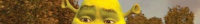
\includegraphics[width=0.9\textwidth]{res/shrek.png}
    \caption{We remove pixels from shrek, $\bm{\bar{x}}$, at random shown in the mask (top), to produce a very sparse version of shrek, $\bm{z}$ (middle). The result of our interpolation and noise reduction is shown, $\bm{\hat{x}}$, (bottom). We observe that the key components of shrek, the facial features, eyes, ears, and eyebrows are successfully recovered through the use of our inpainting technique (10K iterations of our Chambolle-Pock).}
    \label{fig:shrek}
\end{figure}


\subsubsection{Inpainting in Landsat/Sentinel-2 data}
We consider the case where our obtained data is $\bm{z} \in \mathbb{R}^M$ and fitted data is, $\bm{\hat{x}} \in \mathbb{R}^N$, where $N=N_{\text{DGO}}\times N_{time}$ and $M \leq N$ to account for missing data. The final modification of the inpainting procedure is to have the ability to implement different regularisation penalties in both space and time. This is done through implementing the second-derivative in one direction, and the first-derivative in the other along with a seperate scaling parameter, $\lambda_i$, for each dimension. In any case, the modified linear operator is applied in the same way within the Chambolle-Pock method.

\begin{align}
  \bm{\hat{x}} &\in \operatorname{argmin}_{\bm{x} \in \mathbb{R}^N}
  \frac{1}{2}{||A\bm{x}-\bm{z}||^2_2} + \lambda_{\text{DGO}} ||L_{\text{DGO}}\bm{x}||_1
   + \lambda_{\text{time}}||L_{\text{time}}\bm{x}||_1
  \label{eqn:minim-data}
\end{align}

Results are shown in (Figure \ref{fig:shrek-params}) where $L_\text{DGO}$ and $L_\text{time}$ are either a first or second order derivative/difference operators. The first order derivative favours piece-wise constant behaviour, while the second favours piece-wise linear. This technique is then applied to our Landsat (Figure \ref{fig:landsat_3_1_second_first}) and Sentinel-2 data (Figure \ref{fig:sentinel_5_5_second_second}).

\begin{figure}[H]
    \centering
    \includegraphics[width=0.9\textwidth]{res/shrek_params.png}
    \caption{We perform 10K iterations with a different x-axis and y-axis lengthscale. We observe the characteristic 'blockiness' (top image) when we perform L1-regularisation on the first derivative. We clearly see the varying impact of the larger length scale on the x-axis than the y-axis. We observe that the algorithm is more flexible with recovering features for larger length scales when we perform L1-regularisation on the second derivative.}
    \label{fig:shrek-params}
\end{figure}

\begin{figure}[H]
    \centering
    \begin{subfigure}[t]{0.45\textwidth}
        \centering
        {\includegraphics[width=\textwidth]{res/shrek_params_a.png}}
    \end{subfigure}
    \begin{subfigure}[t]{0.45\textwidth}
        \centering
        {\includegraphics[width=\textwidth]{res/shrek_params_b.png}}
    \end{subfigure}
    \caption{A cross-section cut of (Figure \ref{fig:shrek-params}) to compare the case of L1-regularisation in the x-axis of the first (a) and second (b) derivatives. We can see the piece-wise constant and piece-wise linear fits for our incomplete data. The modified inpainting Chambolle-Pock method both removes noise variation and interpolates the data.}
    \label{fig:shrek-params-cut}
\end{figure}

\section{Results and Discussion}

From our interpolated braiding intensity data (Figure \ref{fig:landsat_3_1_second_first}), we see a clear seasonal yearly temporal variation with the braiding intensity rising each June, during monsoon season, and then subsequently falling. This can be attributed to varying precipitation and rainfall. We see that at DGOs 0 to 10 the magnitude of this temporal variation is smaller. This is because of human intervention with neighbouring urban developments, where the maximum extent of the river is confined as it is forced to flow in a single channel. \\

Along the length of our river, from DGO 20 to 40, we view spatial periodicity in our braiding intensity. This is more clearly seen in our Sentinel-2 data (Figure \ref{fig:sentinel_5_5_second_second}), and in our $L=[\text{second},\text{second}]$ plot of (Figure \ref{fig:landsat_3_1_second_first}) as it is smoothed out by our y-axis length scale in the other plot. This can be explained spatial river morphology that is impacted through both environmental and anthropomorphic factors. \\

At DGOs 40 to 50, we observe that the braiding intensity is almost constant and the magnitude of temporal variation is significantly smaller. This can be explained by the existence of the city of Lhasa nearby. \\

At DGO 53 we observe a sharp spatial increase in braiding intensity, this can be explained by the existence of a dam and a dyke beforehand which brings the river into a single channel as it passes through the city of Lhasa, following the Dam the morphology of the river instantly changes back into its subsequent multi-channeled behaviour. \\

Furthermore, we compare the use of different L1-regularisation modes for our y-axis for our Landsat data (Figure \ref{fig:landsat_3_1_second_first}). In the top image we penalise our first y-axis derivative and in the bottom we penalise the second. This is because we expect sharp spatial discontinuities in the behaviour of our river (i.e. if a dam exists) which may be better captured through fitting a piece-wise constant curve. This is clearly seen in DGO 53, where we observe the sharp jump in braiding intensity due to the dam. Unfortunately, this also obscured the spatial variation of braiding index at DGOs 20 to 40. \\

All of these findings are reciprocated and also seen in our Sentinel-2 data (Figure \ref{fig:sentinel_5_5_second_second}). However, our sentinel data reveals a greater magnitude of braiding intensity variation between DGOs 40-50. Further, the magnitude of Braiding Intensity for almost all datapoints is greater. The variations and general behaviour of both the Landsat and Sentinel-2 data correspond to each other, but the intensity values are greater by some scale factor in Sentinel-2. This can be explained by the fact that with a greater resolution of our satellite photos we are more likely to capture smaller sub-channels of our river which contribute to our overall braiding intensity value.

\begin{figure}
    \centering
    \begin{subfigure}[t]{0.95\textwidth}
        \centering
        \includegraphics[width=\textwidth]{res/landsat_3_1_second_first.png}
    \end{subfigure}
    \begin{subfigure}[t]{0.95\textwidth}
        \centering
        \includegraphics[width=\textwidth]{res/landsat_3_1_second_second.png}
    \end{subfigure}
    \caption{Our Chambolle-Pock interpolated Landsat data, where pixel intensity represents braiding intensity. We use two different choices of $\lambda_\text{time} = 3$ and $\lambda_\text{dgo} = 1$, therefore leading to a varying L1-regularisation mode for the space axis.}
    \label{fig:landsat_3_1_second_first}
\end{figure}

\begin{figure}
    \centering
    \begin{subfigure}[t]{0.95\textwidth}
        \centering
        \includegraphics[width=\textwidth]{res/sentinel_5_5_second_second.png}
    \end{subfigure}
    \caption{Our Chambolle-Pock interpolated Sentinel-2 data, where pixel intensity is braiding intensity. Due to the increased noise, because of more datapoints, we must increase our length scale accordingly to view features of interest in our plot.}
    \label{fig:sentinel_5_5_second_second}
\end{figure}

\section{Conclusion}
\subsection{Evaluation of River Data Extraction}
The automated process of obtaining our river indices from the Lhasa river takes $\approx 3$ hours. This is for two key reasons. Firstly, the Google Earth API has a data limit which throttles the speed of execution of our code. Lastly, the code is vectorised and it is not possible for it to be directly restructured due to the limitations by which the Google Earth Engine API works. The image tiles are reloaded and the water mask is recalculated for each seperate DGO index unnecessarily. Since there are on the order of 100 DGOs, this slows down our algorithm by 100 fold. More work is required to fix this limitation. \\

In practice, this method remains preferable over the previous state of the art. Crucially, in this case no human intervention is required and the results are cached into a .csv file once run and the indices need to be extracted from the Google Earth Engine only once. As such, the process of extraction may be run overnight, with the post-processing and further analysis done afterwards in real-time.

\subsection{Evaluation of interpolated river data}
We successfully validate the interpolation methodology applied to our Landsat data by viewing its correspondence with our Sentinel-2 data when attempting to provide explanations for the observed morphology of the river, as such: it would be reasonable to apply the same interpolation scheme proposed to the earlier datapoints from 1980 onwards where we do not have data from other satellites in order to learn about the longer-term behaviour of the river and potentially analyse the impact of climate change over the past 40 years. To further verify the correctness of our interpolattion scheme, we may compare interpolated datapoints to their ground truth values. These values are calculated manually from even higher resolution satellite photographs than the Sentinel-2 image collection. Further work is required to directly and accurately combine the Landsat and Sentinel-2 data. This is because of the fact that the braiding intensity calculation is very sensitive to the resolution of our satellites. This will improve the density of our data without obscuring the temporal behaviour by increasing the discretisation bin size.

A key criticism of our interpolation scheme is that we do not have a methodology to tell whether an interpolated data point is reliable or not. It is clear from (Figure \ref{fig:sentinel_sparsity_discretisation_8}), that the true value of an interpolated datapoint in a large empty region (monsoon season) will be highly inaccurate. This inaccuracy is not conveyed on our plots (Figure \ref{fig:sentinel_5_5_second_second}). This problem can be solved through the use of other techniques, where an uncertainty is also held by each datapoint.

An example of an alternative technique is known as Gaussian Processes\cite{rasmussen}. Our method of interpolation does nothing to exploit the observed temporal periodic behaviour of our braiding index. Furthermore, Gaussian Processes also address this problem through the use of a periodic covariance function, allowing us to also predict and extract the underlying periodicity of the data. With more time, Gaussian Processes may be used and implemented for this purpose. Our uncertainty in our calculated braiding index values may be reduced through downloading all of the satellite data and performing the processing offline rather than on the cloud. This will provide total control over the way in which the river data was processed. In practice, this was untenable given the time constraints. Hundreds of gigabytes of computational power and storage space is required and the images would need to be processed manually to obtain the water masks and braiding indices.

To some extent, the temporal variation in our interpolated indices a consequence of the temporal variation of our missing data. The interpolation scheme does not take the periodic nature of our signal itself into account and as a result large sections of interpolated values are calculated every monsoon season (Figure \ref{fig:sentinel_sparsity_discretisation_8}) for the Sentinel-2 data (Figure \ref{fig:sentinel_5_5_second_second}).

% WAIT FOR BARBARA - GIVING HER TIME INFO TODAY FOR THE COMPARISON OF DATAPOINTS...
% TO WHAT EXTENT IS THE TEMPORAL VARIATION A CONSEQUENCE OF OUR TEMPORAL VARIATION IN MISSING DATA INTERPOLATION?
% Use Sentinel to assess data, tell us how accurate the fit is when we use sentinel as a baseline. (% difference!)
    

% \section{Annex}
% Guide for what to do


\begin{thebibliography}{99}

\bibitem{landsat} U.S. Geological Survey,
  {Landsat Collections Satellite Imagery}
  Satellite imagery, Geo. 2020.
  
\bibitem{sentinel} European Commission (Copernicus), ESA.
  {Sentinel-2 Collections Satellite Imagery}
  Satellite imagery, Geo. 2020.
  
\bibitem{google-earth-engine} N, Gorelick, M. Hancher,
 Google Earth Engine: Planetary-scale geospatial analysis for everyone,
 Remote Sensing of Environment, Vol 202, pp. 18-27, 2017.
 
 \bibitem{geemap} Q. Wu
  {geemap: A Python package for interactive mapping with Google Earth Engine}. 
  The Journal of Open Source Software, 5(51), 2305. 2020.

\bibitem{gee-boothroyd} R. Boothroyd, R. Williams, 
 Applications of Google Earth Engine in fluvial geomorphology for detecting river channel change
 WIREs Water, Vol 8, no 1, 2021

\bibitem{qgis} QGIS Development Team (2022). 
  \emph{QGIS Geographic Information System}.
  Open Source Geospatial Foundation Project. http://qgis.osgeo.org".

\bibitem{pekel} JF. Pekel, A. Cottam, et al.
  {High-resolution mapping of global surface water and its long-term changes.}
  Nature 540, pp 418–422, 2016. https://doi.org/10.1038/nature20584
  
\bibitem{braiding-intensity} R. Egozi, P. Ashmore,
  Defining and Measuring Braiding Intensity.
  Geography Publications. Vol 33. 2008.
  
\bibitem{mndwi} H. Xu
  {Modification of Normalised Difference Water Index (NDWI) to Enhance Open Water Features in Remotely Sensed Imagery.}
  International Journal of Remote Sensing 27, no 14, 2006.

\bibitem{proximal-algorithms} N. Parikh, and S. Boyd,
  Proximal algorithms, Foundations and trends in Optimization,
  Vol 1, no 3, pp. 127-239, 2014.

\bibitem{fixed-point} P.L. Combettes, and J. Pesquet,
  Proximal splitting methods in signal processing, Fixed-point algorithms for inverse problems in science and engineering.
  Springer, New York, NY, 2011.

\bibitem{chambolle-pock} A. Chambolle, T. Pock.
  {A first-order primal-dual algorithm for convex problems with applications to imaging.} (2010).
  J Math Imaging Vis 40, pp. 120–145, 2011.

\bibitem{chambolle-pock-2} A. Chambolle,
  An algorithm for total variation minimization and applications.
  Journal of Mathematical imaging and vision, Vol 20, no 1, pp 89-97, 2004.

\bibitem{pustelnik} J. Colas, N. Pustelnik, C. Oliver, J.-C. Geminard, V. Vidal,
  Nonlinear denoising for solid friction dynamics characterization, 
  Physical Review E, 100, 032803, Sept. 2019.

\bibitem{rasmussen} CE. Rasmussen, and CKI. Williams.
  Gaussian Processes for Machine Learning.
  MIT Press, 2005.
\end{thebibliography}

\end{document}

